\section{Experiment details}
\subsection{Application of Label-Consistent K-SVD on MNIST}
To test, we decided to use the same number of atoms as previously defined: 1024.  Choosing the same number of atoms allows us to compare the results of traditional Sparse Coding with those of LC-KSVD.\\ 
Besides, we decided to take a big $mu$ to promote discriminative power over reconstruction, we took $mu = 5$..\\

Compared to traditional sparse coding, atoms in the Label-Consistent Sparse Coding dictionary look more like of small pencil strokes in the figure \ref{fig:DLCKSVD}. Nevertheless, we can clearly recognize in some atoms a specific number.\\
\begin{figure}[h]
 \centering
 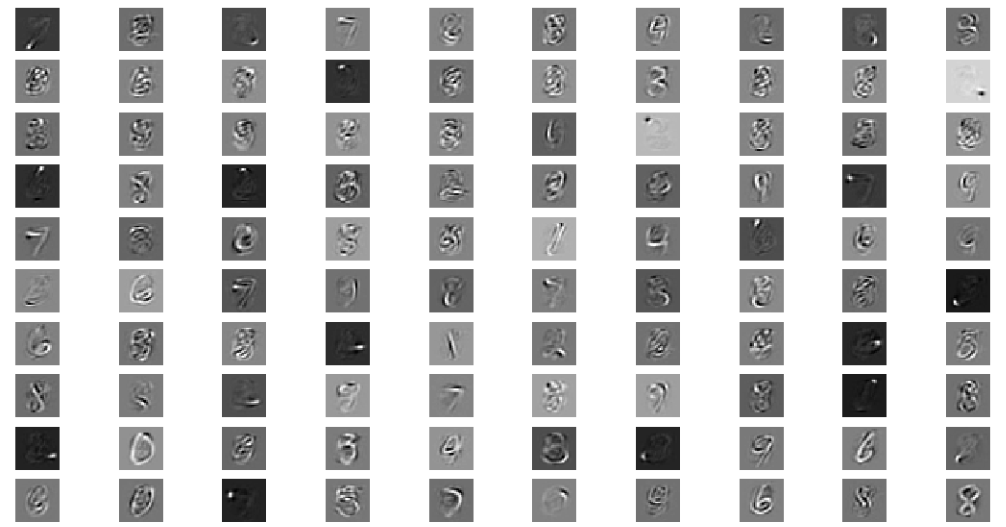
\includegraphics[scale=0.5]{DLCKSVD.png}
 % DLCKSVD.png: 1366x696 px, 100dpi, 34.70x17.68 cm, bb=0 0 984 501
 \caption{Some example of atoms from the dictionary}
 \label{fig:DLCKSVD}
\end{figure}

\begin{figure}[h]
 \centering
 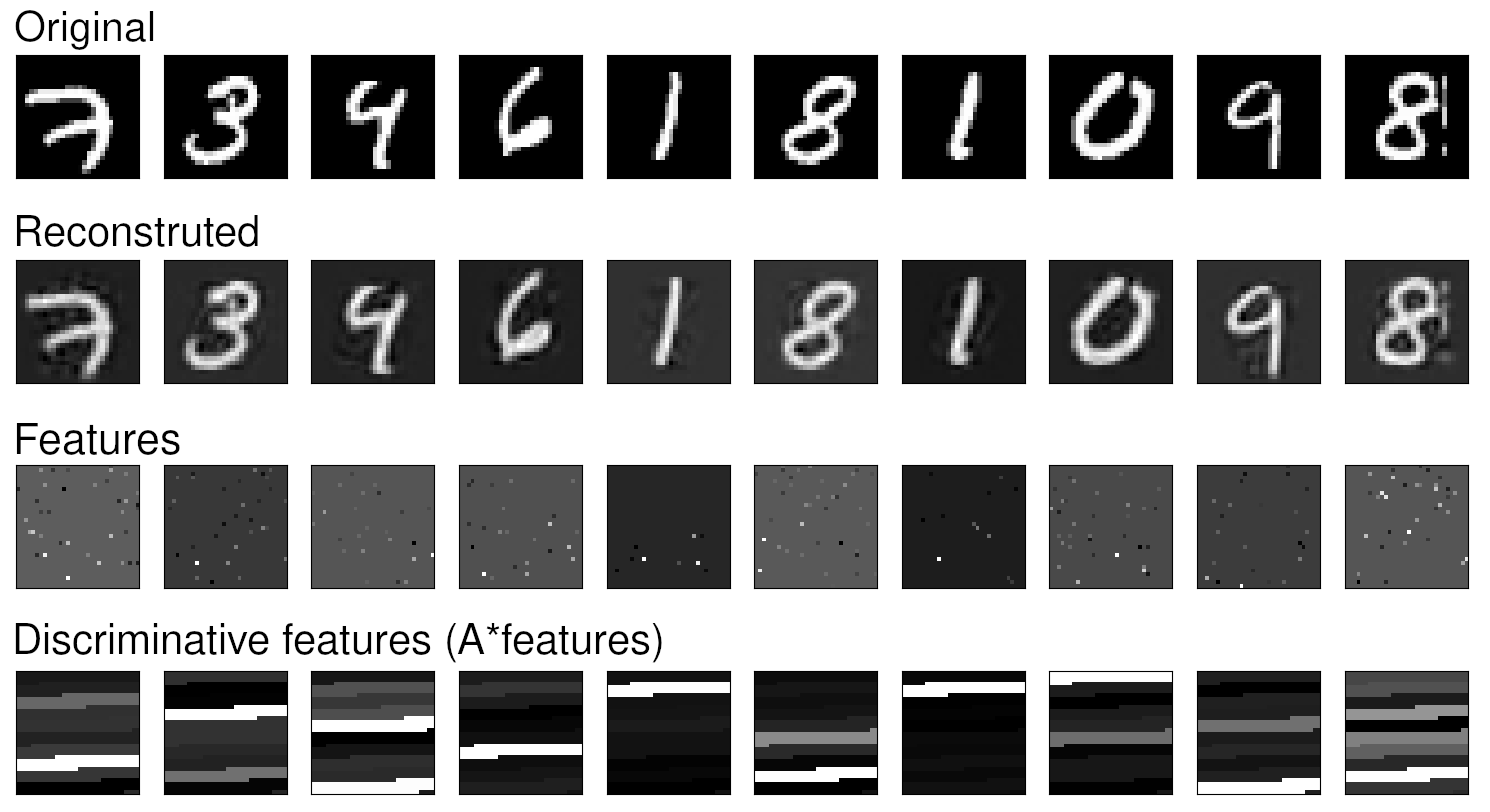
\includegraphics[scale=0.4]{MNIST_LCKSVD.png}
 % MNIST_LCKSVD.png: 1490x812 px, 100dpi, 37.85x20.62 cm, bb=0 0 1073 585
 \caption{Examples of  LC-KVD on MNIST data}
 \label{fig:MNIST_LC}
\end{figure}
Even if we encouraged discrimination more than reconstruction, we can see in the figure \ref{fig:MNIST_LC} that the reconstruction is not bad. In the same figure, we can see that $A * \gamma$ are discriminative: The strongest white band always seem to be in the same location for the same label.\\
We can hope that the classification will be good, even for an unsupervised method like K-means.\\
\subsection{Classification for Label-Consistent K-SVD}
Our results of classification are the following:
\begin{itemize}
 \item K-means accuracy: 0.78
 \item SVM accuracy: 0.91
\end{itemize}
Nevertheless,  even if these results are good, they are applied on a non-shift-invariant dataset. If we use this method directly on speech, for example, we'll get bad results due to this shift-variance of patterns. That is why we used the convolution operation to deal with this problem. The method which merges Sparse Coding and convolution is called \textit{Convolutional Sparse Coding}.
%\begin{figure}[h]
% \centering
% \includegraphics[scale=0.5]{../Results/LC-KSVD_X_ALL_K_1024/repartition_h.png}
 % répartition_h.png: 681x651 px, 100dpi, 17.30x16.54 cm, bb=0 0 490 469
 %\caption{Sparse coefficients repartition}
%\end{figure}
%\begin{figure}[h]
% \centering
% 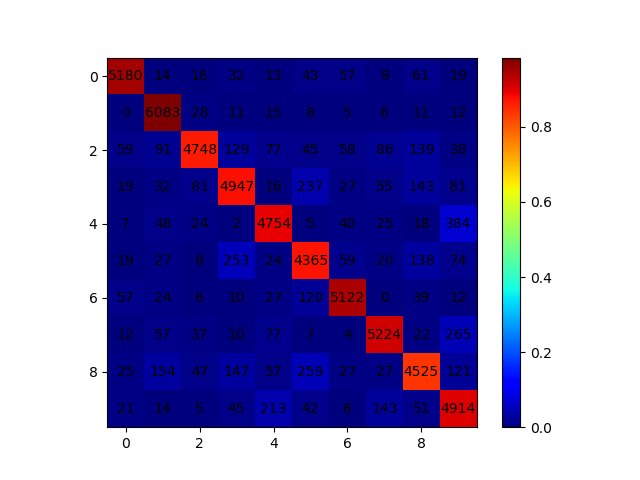
\includegraphics[scale=0.72]{../Results/LC-KSVD_X_ALL_K_1024/confusion_matrix_train.png}
 % confusion_matrix_train.png: 640x480 px, 100dpi, 16.26x12.19 cm, bb=0 0 461 346
% \caption{Kmeans classification on A$\alpha$ from the trainning dataset}
%\end{figure}


% \begin{figure}[h]
 %\begin{subfigure}{.5\textwidth}
 %\centering
 %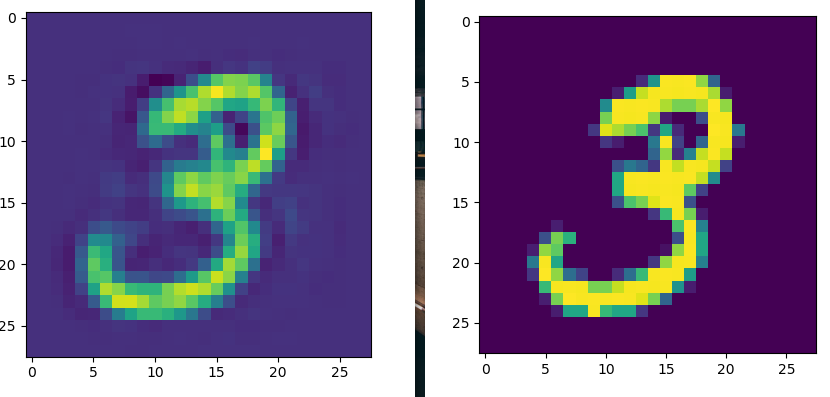
\includegraphics[scale=0.29]{../Results/LC-KSVD_X_ALL_K_1024/3_recons.png}
 % \caption{Reconstructed 3 vs Original 3}
 % module-capteur-laser.jpg: 600x600 px, 72dpi, 21.17x21.17 cm, bb=0 0 600 600
 %\end{subfigure}%
 % \begin{subfigure}{.3\textwidth}
 %\centering
 %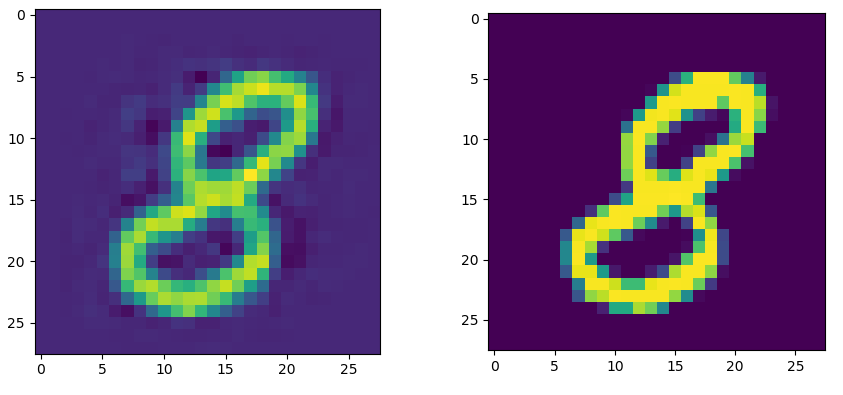
\includegraphics[scale=0.29]{../Results/LC-KSVD_X_ALL_K_1024/8_recons.png}
 % module-capteur-laser.jpg: 600x600 px, 72dpi, 21.17x21.17 cm, bb=0 0 600 600
 % \caption{Reconstructed 8 vs Original }

 %\end{subfigure}%
%\end{figure}

%\begin{figure}[h!]
% \centering
% 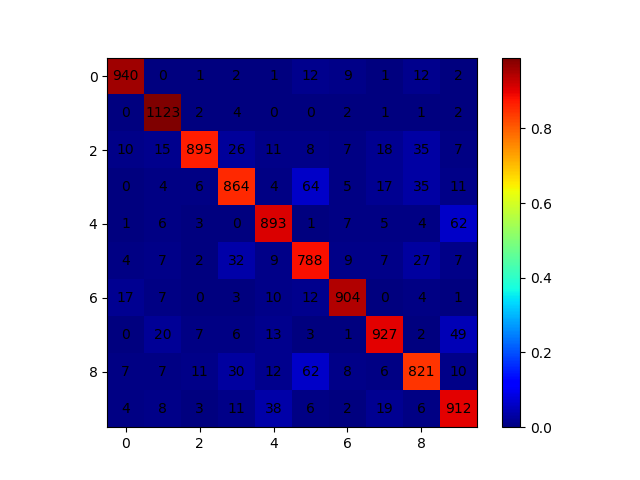
\includegraphics[scale=0.3]{../Results/LC-KSVD_X_ALL_K_1024/confusion_matrix_test.png}
 % confusion_matrix_test.png: 640x480 px, 100dpi, 16.26x12.19 cm, bb=0 0 461 346
% \caption{Kmeans classification on A $\alpha$ from the test dataset w}
%\end{figure}
